\section{Results in three dimensions}\label{sec:results3d}

The three-dimensional comparison is the run of 28 September 2026, made under the
pre-registered amendment of \cref{sec:methods:prereg}; its configuration hash is given in
\ref{app:repro}.

\subsection{The same network with and without labels}\label{sec:results3d:same}

% generated by scripts/make_cmame_material.py from the records; do not edit
\begin{table}[tbp]
\centering
\footnotesize
\setlength{\tabcolsep}{4pt}
\caption{Three-dimensional solids, every metric at the largest label budget. The supervised networks were trained on 1,024 labelled instances; the label-free network on the same 1,024 instances without their solutions.}
\label{tab:3d}
\resizebox{\ifdim\width>\textwidth\textwidth\else\width\fi}{!}{%
\begin{tabular}{lcccccc}
\toprule
Model & \shortstack{Displacement \\ error} & \shortstack{Relative \\ energy gap} & \shortstack{von Mises \\ error} & \shortstack{Peak stress \\ error} & \shortstack{Critical-region \\ recall} & \shortstack{Worse than \\ zero field} \\
\midrule
Label-free & 0.0300 $\pm$ 0.0028 & 0.00912 $\pm$ 0.00228 & 0.0554 $\pm$ 0.0045 & 0.0807 $\pm$ 0.0134 & 0.793 $\pm$ 0.022 & 0/768 \\
Supervised & 0.0470 $\pm$ 0.0038 & 31.2 $\pm$ 53.5 & 0.370 $\pm$ 0.140 & 0.784 $\pm$ 0.807 & 0.619 $\pm$ 0.005 & 18/768 \\
Supervised + energy term & 0.0470 $\pm$ 0.0122 & 0.116 $\pm$ 0.050 & 0.128 $\pm$ 0.008 & 0.115 $\pm$ 0.026 & 0.730 $\pm$ 0.006 & 2/768 \\
Graph network, supervised & 0.0168 $\pm$ 0.0001 & 0.447 $\pm$ 0.084 & 0.296 $\pm$ 0.010 & 0.488 $\pm$ 0.011 & 0.679 $\pm$ 0.009 & 28/768 \\
\midrule
Nearest-neighbour field & 0.382 & 1.22 & 0.717 & 1.23 & 0.509 & 88/256 \\
Scaled polynomial & 1.56 & 4,362 & 14.9 & 54.8 & 0.137 & 256/256 \\
\midrule
Zero field & 1.00 & 1.00 & 1.00 & 1.00 & -- & -- \\
\bottomrule
\end{tabular}}

\smallskip
\begin{minipage}{\linewidth}\footnotesize\raggedright
256 validation instances, never trained on; four load cases each. Errors are relative to the reference finite-element solution, per load case, then averaged over the load cases; the relative energy gap of the zero field is 1. Trained networks: mean $\pm$ sample standard deviation over 3 seeds; the nearest-neighbour field and the scaled polynomial are deterministic.\par
Worse than zero field: instance-seed pairs whose relative energy gap exceeds 1, that is, predictions further from the solution in the energy norm than the zero field.\par
Critical-region recall: the share of the 10\% most stressed elements of the reference solution that are also among the 10\% most stressed of the prediction (higher is better; in every other column lower is better).\par
Run of 28 September 2026.
\end{minipage}
\end{table}


\Cref{tab:3d} gives every metric with 1,024 labelled instances. The label-free transformer
was more accurate than the same transformer trained on the solutions of the same
instances, with or without the energy term, on all five metrics, in the seed mean and in
each of the three seeds. Its displacement error, \numThreeFreeDisp{}, was
\numThreeFreeDispAdvantage{} lower than the supervised transformer's, \numThreeLabDisp{};
its relative energy gap, \numThreeFreeGap{}, was \numThreeAncOverFreeGap{} times lower than
that of the supervised transformer with the energy term, the better of the two supervised
variants; and its von Mises error (\numThreeFreeVm{} against \numThreeLabVm{} and
\numThreeAncVm{}), peak stress error (\numThreeFreePeak{} against \numThreeLabPeak{} and
\numThreeAncPeak{}) and critical-region recall (\numThreeFreeRecall{} against
\numThreeLabRecall{} and \numThreeAncRecall{}) were better. Compared instance by instance
within each seed, the label-free transformer had the lower relative energy gap on
\numPairThreeLabGap{} and \numPairThreeAncGap{} of the \numThreePairs{} instance-seed pairs
against the two supervised variants, the lower von Mises error on \numPairThreeLabVm{} and
\numPairThreeAncVm{}, and the lower displacement error on \numPairThreeLabDisp{} and
\numPairThreeAncDisp{}. Unlike in two dimensions, the label-free transformer was also the
more accurate in displacement. Every three-dimensional network multiplied its output by
$F_{\max}$ (\cref{sec:methods:networks}), and we attribute the difference to this; the
attribution has not been tested.

The supervised transformer's mean relative energy gap, \numThreeLabGapMs{}, is the mean of
three seeds, \numThreeLabGapSeeds{}. The second is dominated by one validation instance,
No.~\numWorstIndex{}, whose supervised prediction in seed \numThreeLabWorstSeed{} had a
relative energy gap of \numThreeLabWorst{}, averaged over its four load cases, with a
displacement error of \numWorstSeedLabDisp{}, a von Mises error of \numWorstSeedLabVm{} and
a peak stress error of \numWorstSeedLabPeak{}. The same instance had the largest relative
energy gap of the supervised transformer in all three seeds. Supervised regression on the
displacement error does not control the energy norm, and with it the stresses: the median
relative energy gap of the supervised transformer, \numThreeLabGapMedian{}, is far below
its mean. The energy term repaired most of this, but not at every budget: with 256 labels
it raised the displacement error of the supervised transformer in every seed and, through
one of the three seeds, its mean relative energy gap, although it reduced the predictions
worse than the zero field from \numThreeLabWorseTwoFiveSix{} to
\numThreeAncWorseTwoFiveSix{} (\cref{tab:labeleff}).

\subsection{Displacement error ranks surrogates in reverse}\label{sec:results3d:reverse}

\begin{figure}[tbp]
\centering
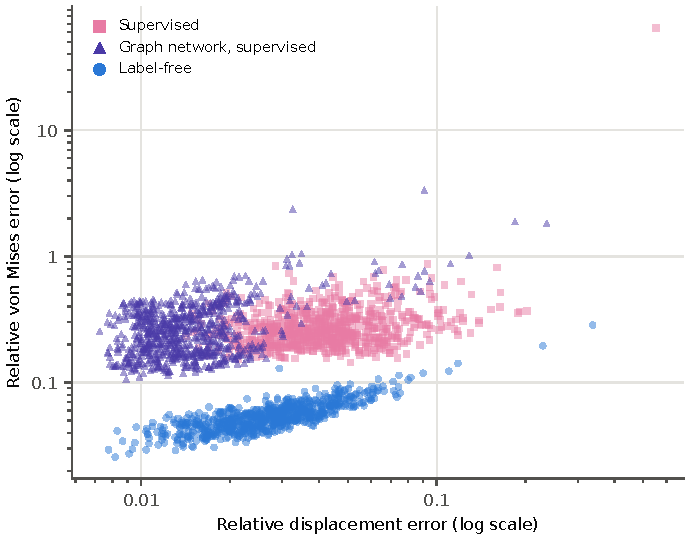
\includegraphics[width=0.72\linewidth]{generated/fig_disp_vs_stress.pdf}
\caption{Three dimensions, 1,024 labelled instances: relative displacement error against
relative von Mises error for every validation instance and seed (\numThreePairs{} points per
network). The graph network's points lie to the left of the label-free transformer's, at
lower displacement error, and above them, at higher stress error. The point at the top
right is instance No.~\numWorstIndex{} in seed \numThreeLabWorstSeed{}
(\cref{sec:results3d:same}).}
\label{fig:reverse}
\end{figure}

The graph network trained with labels had the lowest mean displacement error in
\cref{tab:3d}, \numThreeMgnDisp{}, \numThreeFreeOverMgnDisp{} times lower than the
label-free transformer's, and the label-free transformer was more accurate on every other
metric. The reversal holds on most instances individually (\cref{fig:reverse}). Compared
within each
seed, the graph network's displacement error was lower on \numMgnDispLowerMin{} to
\numMgnDispLowerMax{} of the instances, but its von Mises error was higher on
\numMgnVmHigher{} of the \numThreePairs{} instance-seed pairs, with a mean
\numThreeMgnOverFreeVm{} times higher, and its relative energy gap was higher on at least
\numMgnGapHigherMin{} of the instances in every seed. On \numMgnLowerDispHigherVm{} pairs
both held at once: a lower displacement error and a higher stress error. The peak stress
error, which compares a single value per load case, follows the pattern less closely: the
graph network's was the lower on \numMgnPeakLowerMin{} to \numMgnPeakLowerMax{} of the
instances, although its mean was \numThreeMgnOverFreePeak{} times higher.

Validation instance No.~\numWorstIndex{} in seed 0 (\cref{fig:field-worst}) shows the
pattern on one instance. The label-free transformer had the largest displacement error of
the three networks, \numWorstFreeDisp{}, and the most accurate stresses, with a von Mises
error of \numWorstFreeVm{} and a relative energy gap of \numWorstFreeGap{}. The supervised
transformer and the graph network had displacement errors of \numWorstLabDisp{} and
\numWorstMgnDisp{}, von Mises errors of \numWorstLabVm{} and \numWorstMgnVm{}, and relative
energy gaps of \numWorstLabGap{} and \numWorstMgnGap{}: both were more accurate in
displacement and worse than the zero field in energy. \Cref{fig:field-median} shows a
typical instance. \Cref{rem:rank} shows that such reversals are possible only when the
displacement errors differ by less than $\kappa^{1/2}$, and \cref{prop:stress} why the
energy, not the displacement, follows the stress.

\begin{figure}[tbp]
\centering
\pending{Field plot of validation instance No.~\numWorstIndex{}, seed 0: magnitude of the
displacement (top) and von Mises stress (bottom) of the reference solution and the three
networks, with the sign of $\Pi_h(u)$ for each network. The fields are exported on the
training machine together with the cost measurements of \cref{sec:cost}.}
\caption{Validation instance No.~\numWorstIndex{}, seed 0 (selection rule in
\cref{sec:methods:prereg}).}
\label{fig:field-worst}
\end{figure}

\begin{figure}[tbp]
\centering
\pending{Field plot of the validation instance with the median relative energy gap of the
label-free transformer, seed 0: von Mises stress of the reference solution, the
label-free transformer and the graph network.}
\caption{A typical validation instance, seed 0 (selection rule in
\cref{sec:methods:prereg}).}
\label{fig:field-median}
\end{figure}

\subsection{Failures and their detection}\label{sec:results3d:detection}

\begin{figure}[tbp]
\centering
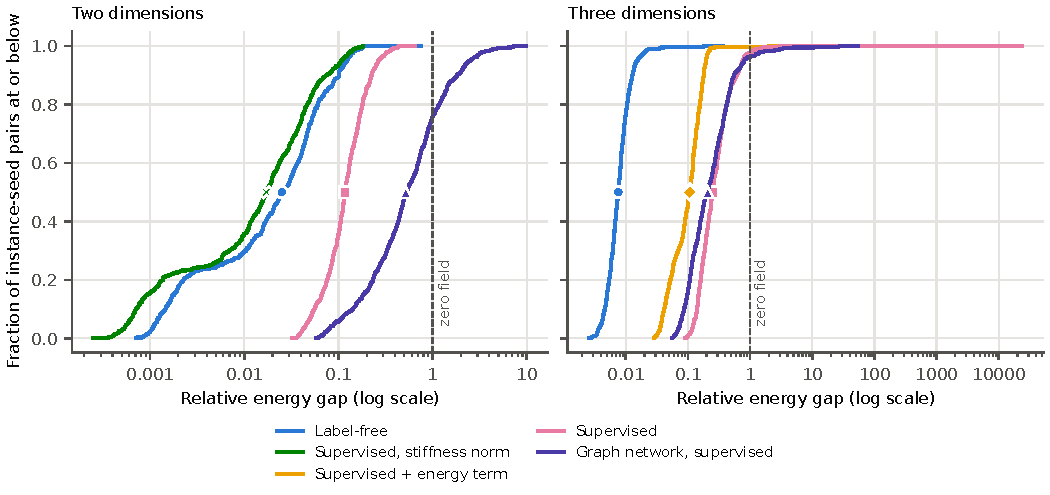
\includegraphics[width=\linewidth]{generated/fig_energy_gap.pdf}
\caption{Distribution of the relative energy gap over the \numThreePairs{} validation
instance-seed pairs, 1,024 labelled instances, in two dimensions (left) and three
dimensions (right). Markers show the medians; predictions to the right of the dashed line
are further from the solution, in the energy norm, than the zero field.}
\label{fig:energygap}
\end{figure}

\Cref{fig:energygap} shows the distribution of the relative energy gap. In three
dimensions the label-free transformer's median, \numThreeFreeGapMedian{}, was
\numThreeMedianRatioMin{} to \numThreeMedianRatioMax{} times lower than the supervised
networks' medians, and none of its \numThreePairs{} instance-seed predictions had a mean
relative energy gap above one. The supervised transformer had \numThreeLabWorse{} such
predictions, the supervised transformer with the energy term \numThreeAncWorse{} and the
graph network \numThreeMgnWorse{}. Per load case, the readings of
\cref{sec:transfer:amplitude} give the label-free transformer \numThreeFreeLoadWorse{}
prediction worse than the zero field among \numThreeFreeLoads{}.
\pending{Per-load-case counts for the supervised networks, from the energies exported on
the training machine.}

None of these failures needs a reference solution to be found. By \cref{cor:zero}, a load
case whose prediction is worse than the zero field is exactly one with $\Pi_h(u)>0$, which
is known as soon as the energy has been evaluated; by \cref{prop:amp}, rescaling by $\cstar$
turns it into a prediction no worse than the zero field. The check applies to any network,
however it was trained; for the label-free transformer the energy is also the training
objective.

\subsection{Label efficiency}\label{sec:results3d:labels}

In three dimensions (\cref{tab:labeleff,fig:labeleff}, right) the label-free
transformer's relative energy gap was lower than every supervised network's at every
budget, and its displacement error lower than both supervised transformers' at every
budget. The graph network reached a lower displacement error than the label-free
transformer with 1,024 labels, not with 64. The supervised transformer's relative energy
gap did not fall monotonically with the number of labels: its seed mean rose from 256 to
1,024 labels, through the single instance discussed in \cref{sec:results3d:same}.

\subsection{Pre-registered decisions}\label{sec:results3d:decisions}

The gate of this run combined three conditions as (a) and ((b) or (c))
(\cref{tab:criteria}). Condition (a)
is a sanity check on the supervised side: the supervised transformer with the energy term
must be at least \numGTwoSanityX{} times more accurate in displacement than the zero field
and better than both naive baselines. Condition (b) concerns the label-free transformer:
its displacement error within 10\% of the supervised transformer's with 1,024 labels, and
an advantage in relative energy gap of at least 40\% at every budget. Condition (c)
concerns transfer to the finer mesh.

Condition (b) was met with a wide margin: the label-free displacement error was
\numGTwoParity{} relative to the supervised one, and the smallest advantage in relative
energy gap was \numGTwoAdvMin{}. Condition (c) failed (\cref{sec:transfer}), and kill
condition KP4 withdrew the transfer claim. Condition (a) was met at 64, 256 and 1,024
labels, by factors of \numGTwoSanitySixtyFour{} to \numGTwoSanityMax{}, but not at 16
labels, where the factor was \numGTwoSanitySixteen{}. The amendment of
\cref{sec:methods:prereg} assessed (a) only from \numGTwoFloor{} labels on; under it the
gate read GO, under the registered form, which assesses every budget, NO-GO. Condition (a)
involves only the supervised networks and the baselines, whose results were known when the
amendment was written, so the change of reading was made with knowledge of its effect; it
was disclosed in the amendment itself, and the reference reading was computed and published
with the run. The conclusions of this paper rest on condition (b) and on the measurements
themselves, not on the gate's verdict.
